\section{Auswertung}

\subsection*{Vorbemerkungen}

Sofern nicht anders angegeben, berechnen wir die Fehler zusammengesetzter Werte anhand der standardmäßigen Gauß'schen Fehlerfortpflanzung. Die $\sigma$-Abweichung zweier fehlerbehafteter Werte $x \pm \Delta x$ und $y \pm \Delta y$ berechnen wir anhand der Formel
\begin{align}
  \sigma = \frac{\qty|x - y|}{\sqrt{\Delta x^2 + \Delta y^2}}.
\end{align}

Für die Breite des Analysierspalts, abgelesen von der Messuhr, verwedenen wir einen konstanten Fehler von $\pm0.01\si{\milli\meter}$. Für abgelesene Pixelwerte nehmen wir mit einem Fehler von $\pm 4$px an.

\subsection{Eichung der Abszisse}

Wir beginnen die Auswertung der Ergebnisse mit der Eichung der Abszisse, bestimmen also einen Faktor, um im weiteren Verlauf der Rechnungen Pixel in Millimeter umrechnen zu können. Hierzu tragen wir zunächst die Abstände der links- und rechtsseitigen Minima von der fünften bis zur ersten gegen die Breite des Analysierspalts, zu welcher diese gerade noch sichtbar waren, auf.

\begin{table}[H]
  \centering
  \caption{Abstände der Minima 1. bis 5. Ordnung mit zugehöriger Spaltbreite des Analysierspalts}
  \vspace*{0.5em}
  \begin{tabular}{c|c|c|c}
    Ordnung & Pixel (l) $\to$ Pixel (r) [px] & Abstand [px] & Spaltbreite [mm]\\\hline
    5 & $338 \pm 4 \to 1263 \pm 4$ & $925 \pm 6$ & $0.79 \pm 0.01$\\
    4 & $438 \pm 4 \to 1164 \pm 4$ & $726 \pm 6$  & $0.59 \pm 0.01$\\
    3 & $507 \pm 4 \to 1075 \pm 4$ & $568 \pm 6$ & $0.48 \pm 0.01$\\
    2 & $609 \pm 4 \to 984 \pm 4$ & $375 \pm 6$ & $0.30 \pm 0.01$\\
    1 & $689 \pm 4 \to 890 \pm 4$ & $201 \pm 6$ & $0.16 \pm 0.01$
  \end{tabular}
\end{table}

\abbref{fig:abszisseneichung} zeigt die Breiten des Analysierspalts über den jeweiligen Pixelwerten. An die Messdaten fitten wir eine standardmäßige lineare Funktion der Form
\begin{align}
  f(x;a,b) = ax + b.
\end{align}

Die aus dem Fit resultierenden optimierten Werte von $a$ und $b$ lauten
\begin{align}
  a &= (8.63 \pm 0.18) \cdot 10^{-4} \frac{\si{\milli\meter}}{\mathrm{px}},\\[1em]
  b &= -0.018 \pm 0.011 \si{\milli\meter}.
\end{align}

Die Steigung $a$ werden wir fortan als Umrechnungsfaktor verwenden, es gilt also
\begin{align}
  1\mathrm{px} = (8.63 \pm 0.18) \cdot 10^{-4}\si{\milli\meter}.
\end{align}
Zur Verbesserung der Genauigkeit verwenden wir hierbei nicht den hier angegebenen gerundeten Wert, sondern den ungerundeten, nur durch die Genauigkeit des \texttt{float}-Datentyps begrenzten Wert.

\begin{figure}[H]
  \centering
  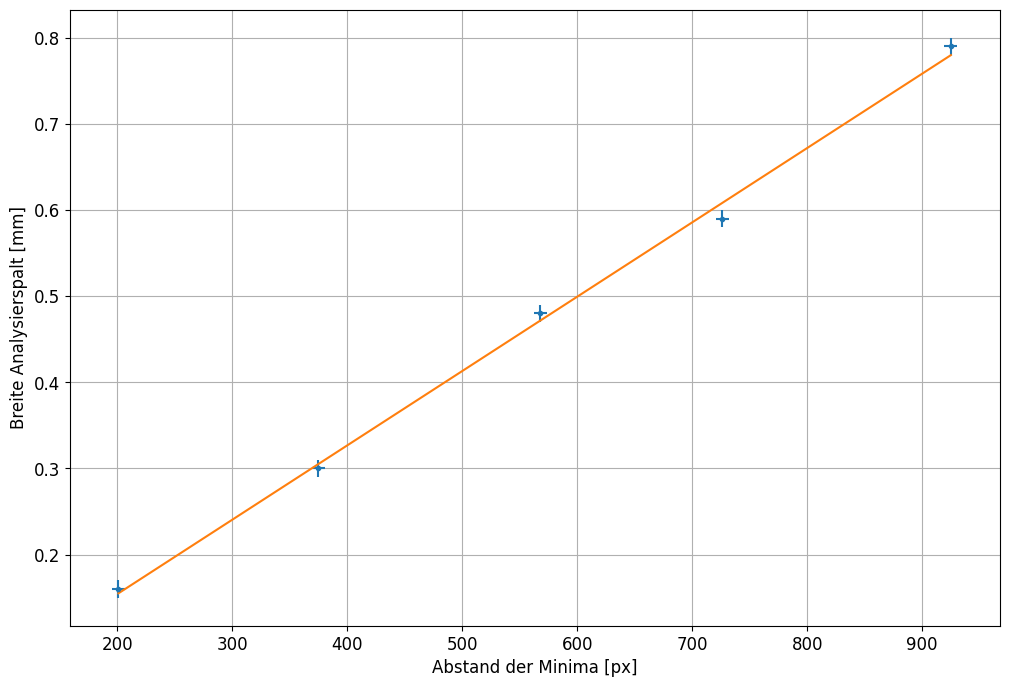
\includegraphics[width=.9\textwidth]{files/plots/2/abszisseneichung.png}
  \caption{Pixel-Abstände über Spaltbreite zur Abszisseneichung}
  \label{fig:abszisseneichung}
\end{figure}
\newpage
\subsection{Quantitative Untersuchung der Beugung am Einzelspalt}

Wir entnehmen zunächst die Positionen der links- und rechtsseitigen Minima erster bis fünfter Ordnung aus den Intensitätsverteilungen. Zunächst aus der, in welcher das Hauptmaximum nicht in Sättigung ist (\abbref{fig:es_nicht_saett_extrema}), dann aus der Verteilung, in welcher das Hauptmaximum in Sättigung ist und die weiter außen liegenden Maxima ebenfalls sichtbar sind (\abbref{fig:es_saett_extrema}). Die Positionen sind in \tabref{tab:es_abst_minima} zusammengefasst. Außerdem ist hier direkt deren Abstand für die weiteren Berechnungen ausgerechnet.

\begin{table}[H]
  \centering
  \caption{Abstände der linksseitigen (l) und rechtsseitigen (r) Minima 1. bis 5. Ordnung}
  \vspace*{0.5em}
  \begin{tabular}{c|c|c}
    Ordnung & Pixel (l) $\to$ Pixel (r) [px] & Abstand [px]\\\hline
    5 & $324 \pm 4 \to 1264 \pm 4$ & $940 \pm 6$\\
    4 & $415 \pm 4 \to 1169 \pm 4$ & $754 \pm 6$\\
    3 & $510 \pm 4 \to 1075 \pm 4$ & $565 \pm 6$\\
    2 & $603 \pm 4 \to 979 \pm 4$ & $376 \pm 6$\\
    1 & $696 \pm 4 \to 885 \pm 4$ & $189 \pm 6$
  \end{tabular}
  \label{tab:es_abst_minima}
\end{table}

Zusätzlich entnehmen wir den Daten noch die Positionen der links- und rechtsseitigen Maxima erster bis fünfter Ordnung, gleichermaßen zusammengefasst in \tabref{tab:es_abst_maxima}.

\begin{table}[H]
  \centering
  \caption{Abstände der linksseitigen (l) und rechtsseitigen (r) Maxima 1. bis 5. Ordnung}
  \vspace*{0.5em}
  \begin{tabular}{c|c|c}
    Ordnung & Pixel (l) $\to$ Pixel (r) [px] & Abstand [px]\\\hline
    5 & $273 \pm 4 \to 1305 \pm 4$ & $1032 \pm 6$\\
    4 & $371 \pm 4 \to 1210 \pm 4$ & $839 \pm 6$\\
    3 & $464 \pm 4 \to 1118 \pm 4$ & $654 \pm 6$\\
    2 & $559 \pm 4 \to 1021 \pm 4$ & $462 \pm 6$\\
    1 & $660 \pm 4 \to 924 \pm 4$ & $264 \pm 6$
  \end{tabular}
  \label{tab:es_abst_maxima}
\end{table}

\begin{figure}[H]
  \centering
  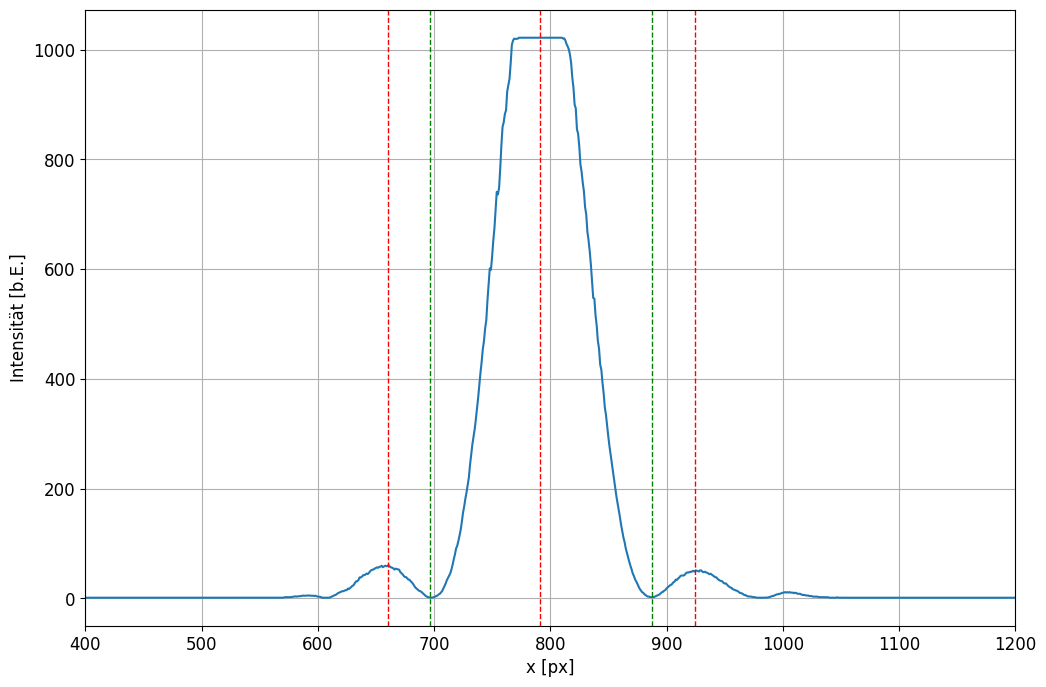
\includegraphics[width=.9\textwidth]{files/plots/2/es_nicht_saett_extrema.png}
  \caption{Intensitätsverteilung bei Beugung am Einzelspalt mit Hauptmaximum nicht in Sättigung}
  \label{fig:es_nicht_saett_extrema}
\end{figure}

\begin{figure}[H]
  \centering
  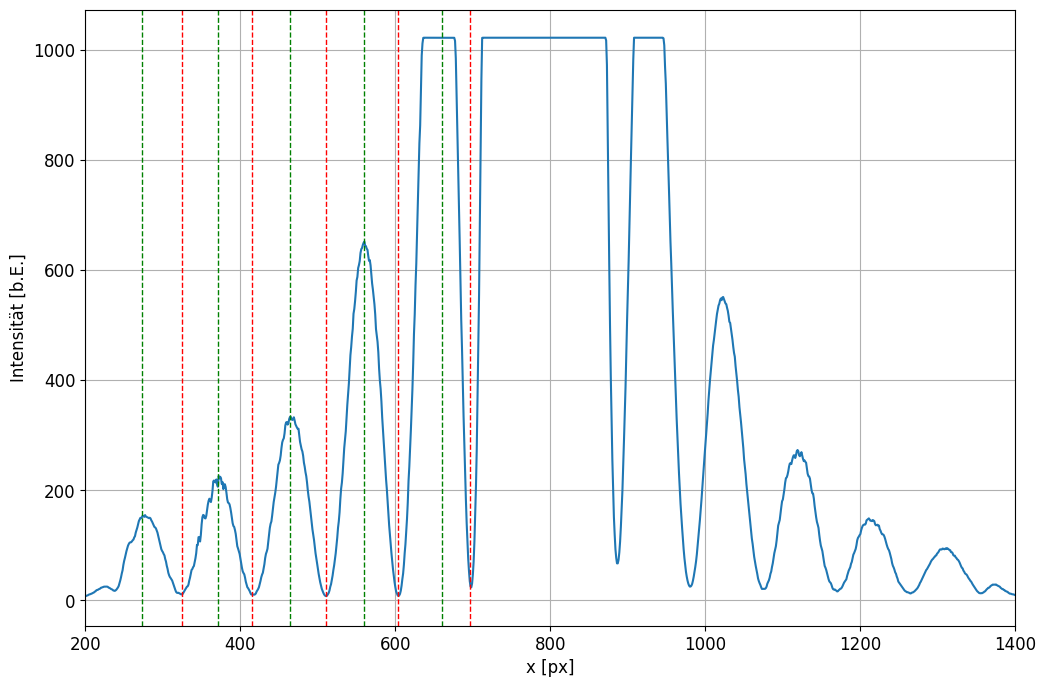
\includegraphics[width=.9\textwidth]{files/plots/2/es_saett_extrema.png}
  \caption{Intensitätsverteilung bei Beugung am Einzelspalt mit Hauptmaximum in Sättigung}
  \label{fig:es_saett_extrema}
\end{figure}

Die Abstände der Minima tragen wir nun über der jeweiligen Ordnung in ein Diagramm auf, zu sehen in \abbref{fig:es_fit_ordnung_ohne_maxima}, und fitten an diese Datenpunkte erneut eine lineare Funktion (diesmal ohne y-Abschnitt, da es sich um eine Ursprungsgerade handelt), um die Steigung zu ermitteln. Hierbei erhalten wir den Wert
\begin{align}
  a &= 188.2 \pm 0.8 \si{\milli\meter}.
\end{align}

Diesen können wir nun verwenden, um eine zwei weitere Aufgabenstellungen zu bearbeiten.

\begin{figure}[H]
  \centering
  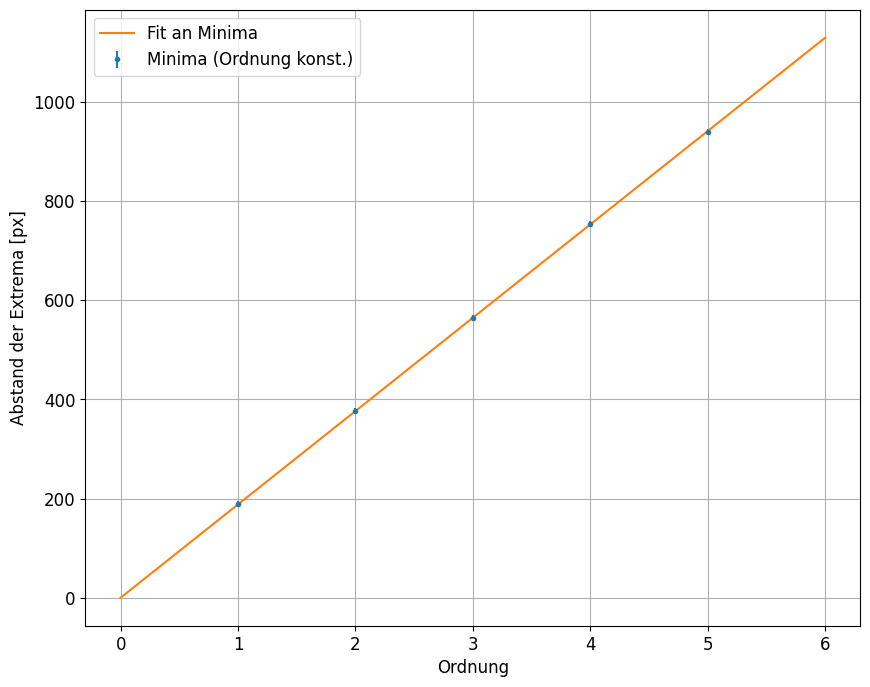
\includegraphics[width=.9\textwidth]{files/plots/2/es_fit_ordnung_ohne_maxima.png}
  \caption{Ordnungen gegenüber der Abstände der jeweiligen Minima mit linearem Fit.}
  \label{fig:es_fit_ordnung_ohne_maxima}
\end{figure}

\subsubsection*{Berechnung der Spaltbreite}

Aus den Grundlagen der Beugung am Einzelspalt wissen wir, dass für den Winkel $\alpha_n$ eines Minimums $n$-ter Ordnung der Zusammenhang
\begin{align}
  b \cdot \sin(\alpha_n) = n \cdot \lambda
\end{align}
mit der Spaltbreite $b$ und der Wellenlänge $\lambda$ des einfallenden Lichts gilt. Weiter können wir aus geometrischen Überlegungen des Versuchsaufbaus herleiten, dass für die Position $x_n$ des $n$-ten Minimums auf dem Schirm in Abstand $d$
\begin{align}
  \tan(\alpha_n) = \frac{x_n}{d}
\end{align}
gilt. Da wir in unserem Aufbau den Schirm genau in der Brennweite $f$ der Sammellinse positioniert haben gilt für uns $d = f$. Für kleine $\alpha_n$ gilt $\sin(\alpha_n) \approx \alpha_n \approx \tan(\alpha_n)$, somit können wir die oberen beiden Gleichungen zusammenfassen zu
\begin{align}
  \frac{n\lambda}{b} = \frac{x_n}{f},
\end{align}
welche wir zur Spaltbreite $b$ umformen können:
\begin{align}
  b = \frac{f \lambda}{\frac{x_n}{n}}.
\end{align}
Der Bruch $\frac{x_n}{n}$ entspricht dabei genau der Steigung $a$ der Gerade, welche wir gerade eben an die Abstände der Minima gefittet haben. Somit haben wir mit
\begin{align}
  b = \frac{f\lambda}{a}
\end{align}
eine Formel für die Spaltbreite hergeleitet. In diese setzen wir die Wellenlänge des Laserlichts von $\lambda = 532 \cdot 10^{-6} \si{\milli\meter}$, die Brennweite $f = 80 \pm 2 \si{\milli\meter}$, sowie die zuvor bestimmte Steigung, welche wir zuvor mit dem Umrechnungsfaktor in Millimeter umrechnen, ein. Wir erhalten damit eine Spaltbreite von
\begin{align}
  b = (0.262 \pm 0.007)\si{\milli\meter}.
\end{align}

\subsubsection*{Bestimmung der Ordnungen der Nebenmaxima}

Das Verhältnis der Ordnungen der Nebenmaxima zu ihren Abständen sollte dem gleichen proportionalen Verhältnis folgen, wie das der Nebenminima. Um dies zu bestätigen, stellen wir das proportionale Verhältnis um, um vom Abstand der links- und rechtsseitigen Maxima auf ihre Ordnung schließen zu können. 

\begin{align}
  \mathrm{ord}_{\max} = \frac{\mathrm{Abstand}_{\max}}{\mathrm{Steigung}}
\end{align}
Die Resultate der Berechnungen sind in \tabref{tab:es_maxima_ord_ber_vergl} zusammengefasst und auch in \abbref{fig:es_fit_ordnung} gegen die Abstände aufgetragen. An den Zahlenwerten sehen wir, dass die Ordnungen immer in etwa zwischen den ganzen Zahlen der Ordnungen der Minima liegen, was sich auch grafisch in \abbref{fig:es_fit_ordnung} bestätigen lässt.

Um diese Werte noch mit den theoretischen Vorhersagen zu vergleichen, betrachten wir die Maxima der sinc-Funktion. Wir in den theoretischen Grundlagen erklärt, gilt für die Intensitätsverteilung des Beugungsbildes des Einzelspalts
\begin{gather}
  I(k_y) = F(k_y)^2 = \sinc(\frac{k_y d}{2})^2 d^2
  \intertext{mit Nullstellen bei}
  k_y = \frac{2\pi n}{d}.
\end{gather}
Setzen wir dies in die Gleichung oben ein, so erhalten wir
\begin{align}
  I(n) = \sinc(n\pi)^2 d^2,
\end{align}
wobei wir den Faktor $d^2$ vernachlässigen können, da es uns nur um die $x$-Positionen der Extrema geht. Die Maxima bestimmen wir, indem wir die Funktion in den Online-Grafikrechner \texttt{Desmos} eingeben und diese ablesen, wie in \abbref{fig:maxima_normed_sinc} zu sehen. Die Abweichung von den Berechneten werten bestimmen wir anhand der $\sigma$-Abweichung mit dem Fehler der berechneten Ordnung.

\begin{table}[H]
  \centering
  \caption{Abstände der linksseitigen (l) und rechtsseitigen (r) Maxima, die berechneten Ordnungen und Vergleich zu den theoretischen Vorhersagen.}
  \vspace*{0.5em}
  \begin{tabular}{c|c|c|c|c}
    Pixel (l) $\to$ Pixel (r) [px] & Abstand [px] & Ber. Ord. & Theo. Ord. & Abweichung\\\hline
    $273 \pm 4 \to 1305 \pm 4$ & $1032 \pm 6$ & $5.48 \pm 0.04$ & $5.48$ & $0$\\
    $371 \pm 4 \to 1210 \pm 4$ & $839 \pm 6$ & $4.46 \pm 0.04$ & $4.48$ & $0.5\sigma$\\
    $464 \pm 4 \to 1118 \pm 4$ & $654 \pm 6$ & $3.48 \pm 0.04$ & $3.47$ & $0.25\sigma$\\
    $559 \pm 4 \to 1021 \pm 4$ & $462 \pm 6$ & $2.46 \pm 0.04$ & $2.46$ & $0$\\
    $660 \pm 4 \to 924 \pm 4$ & $264 \pm 6$ & $1.40 \pm 0.04$ & $1.43$ & $0.75\sigma$
  \end{tabular}
  \label{tab:es_maxima_ord_ber_vergl}
\end{table}

\begin{figure}[H]
  \centering
  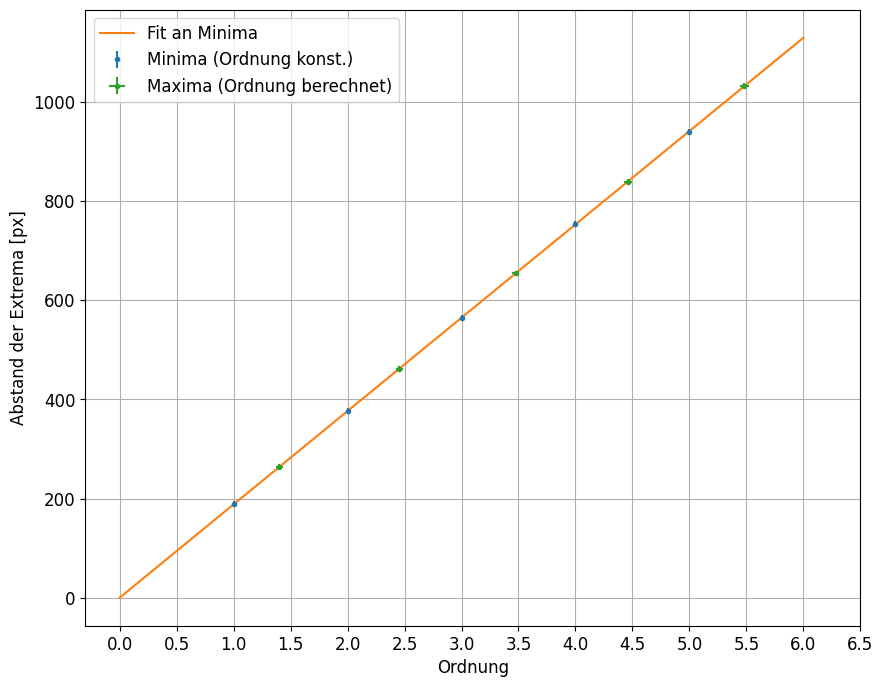
\includegraphics[width=.9\textwidth]{files/plots/2/es_fit_ordnung.png}
  \caption{Ordnungen gegenüber der Abstände der jeweiligen Minima mit linearem Fit und berechnete Ordnungen der Maxima.}
  \label{fig:es_fit_ordnung}
\end{figure}

\begin{figure}[H]
  \centering
  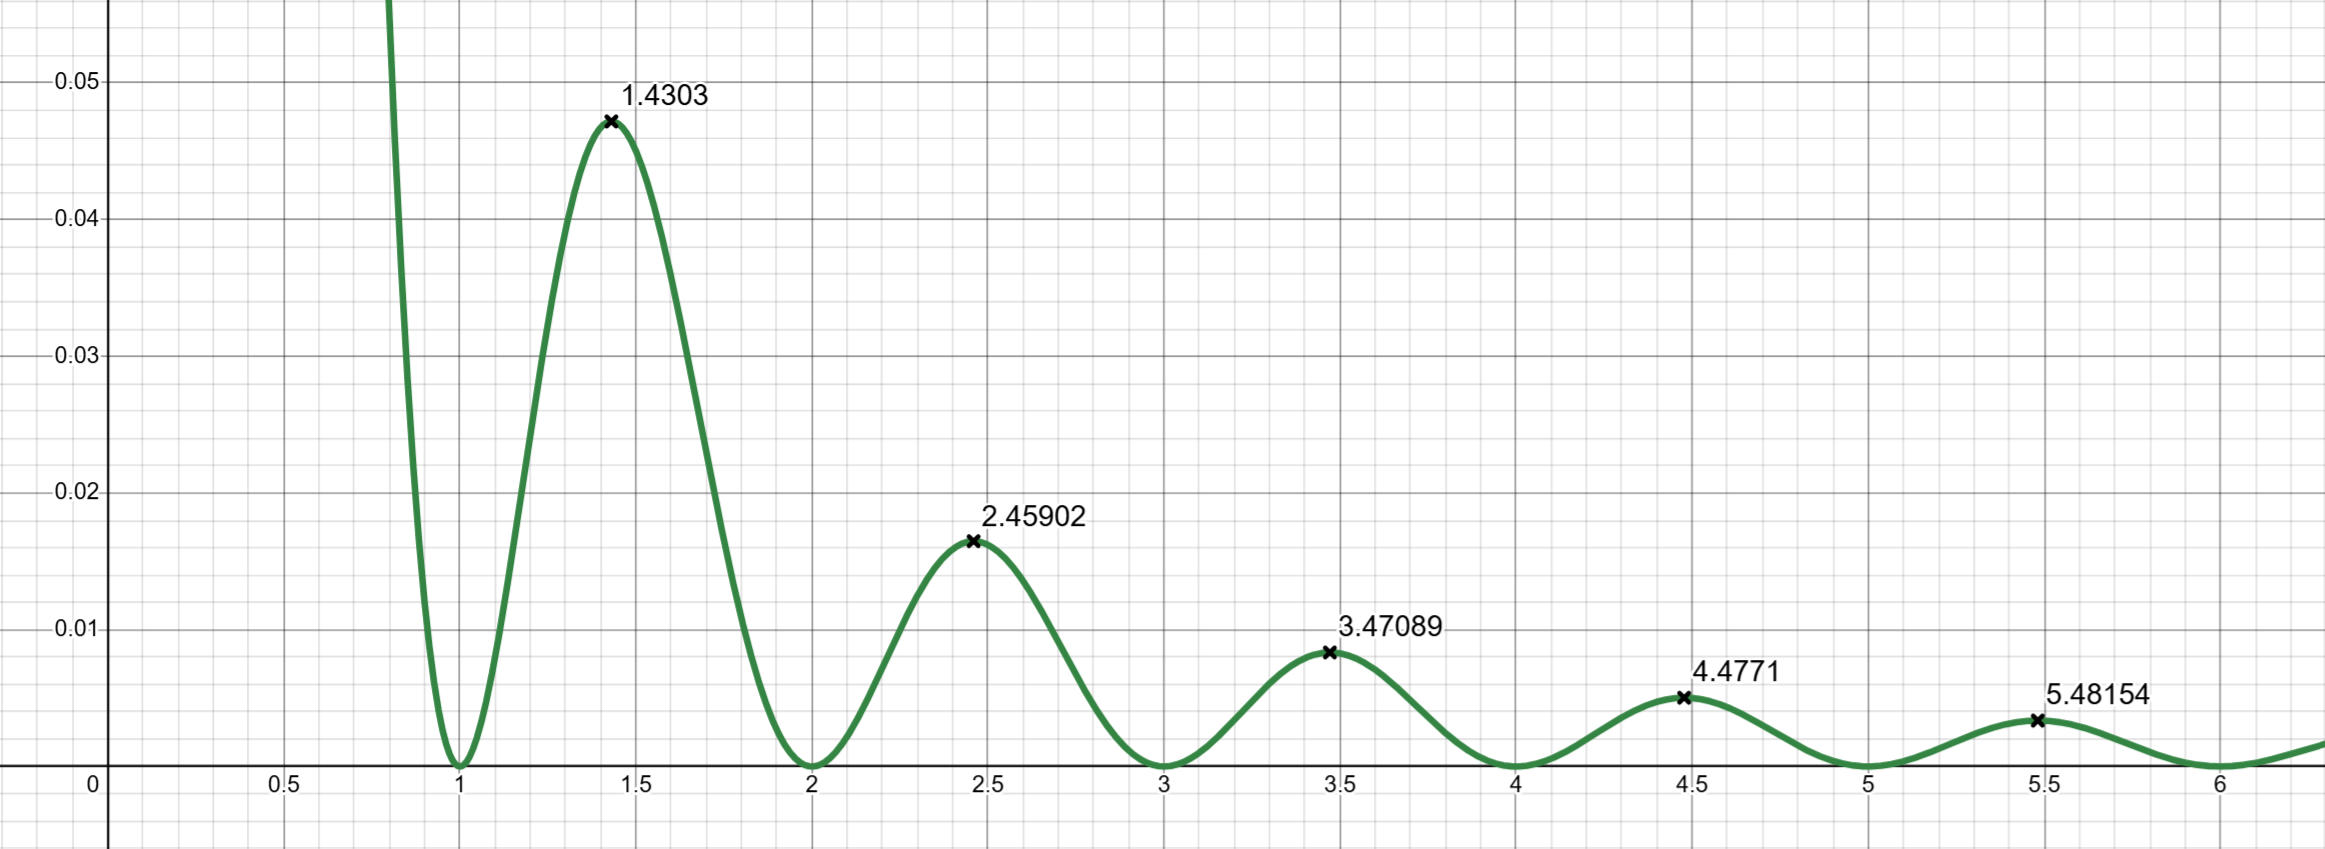
\includegraphics[width=\textwidth]{files/plots/2/maxima_normed_sinc.png}
  \caption{Maxima der normierten sinc-Funktion.}
  \label{fig:maxima_normed_sinc}
\end{figure}

\subsubsection*{Vergleich der Intensitäten}

An dieser Stelle der Auswertung würden wir die Intensitäten der Maxima in den Aufgezeichneten Beugungsbildern mit den theoretisch erwarteten Beugungsbildern vergleichen. Wie allerdings bereits auf den Abbildungen \ref{fig:es_nicht_saett_extrema} und \ref{fig:es_saett_extrema} zu sehen ist, ist uns bei der Aufzeichnung der Intensitätsverteilungen ein Fehler unterlaufen, sodass die Maxima 0. und 1. Ordnung bereits sehr stark in Sättigung sind. Möglicherweise war hier die Belichtungszeit bereits bei der Aufnahme mit der Kamera zu hoch eingestellt, oder wir hatten beim Export über \texttt{Gwyddeon} eine falsche Einstellung gewählt. 

Theoretisch würden wir wie folgt vorgehen: Anhand der Intensität 0. Maximums und der Beachtung der verschiedenen Belichtungszeiten können wir die beiden Intensitätsverteilung normieren, sodass wir einen verhältnismäßigen Abstieg der Maxima 1. bis 5. Ordnung im Vergleich zum Maximum 0. Ordnung erhalten.

Dann generieren wir ein theoretisches Beugungsbild anhand des in der Praktikumsanleitung bereitgestellten Skripts, wie sie in \abbref{fig:es_theorie_beugungsbild} zu sehen ist.

\begin{figure}[H]
  \centering
  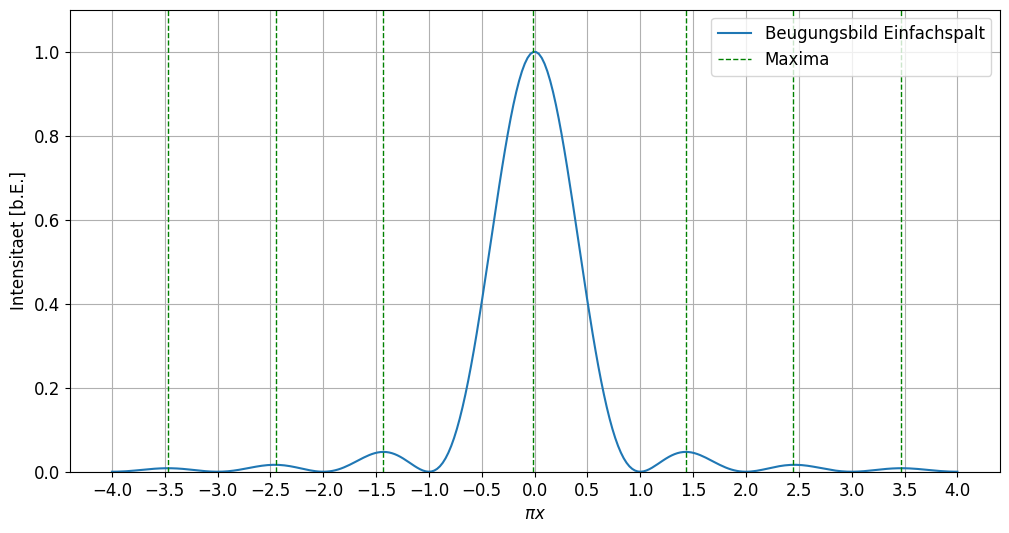
\includegraphics[width=.9\textwidth]{files/plots/2/es_theorie_beugungsbild.png}
  \caption{Theoretisches Beugungsbild des Einzelspalts.}
  \label{fig:es_theorie_beugungsbild}
\end{figure}

In diesem Beugungsmuster sind die Intensitäten ebenfalls anhand der Intensität des Maximums 0. Ordnung normiert. Nun können wir diese auslesen, entweder mit numerischen Methoden in Python oder wieder anhand von einem Online-Grafikrechner, und anschließend mit den gemessenen, normierten Intensitäten vergleichen.

\subsection{Quantitative Untersuchung der Beugung am Doppelspalt}

Einleitend zu dieser Aufgabe haben wir qualitativ die Auswirkungen verschiedener Geometrien des Doppelspalts betrachtet. Dazu waren auf dem Dia drei verschiedene Doppelspalte, in drei verschiedenen Breiten, angebracht.

Auf dem Beugungsbild des breitesten Doppelspalts, zu sehen in \abbref{fig:breit} konnten wir deutlich das mittlere Hauptmaximum mit drei bis view Nebenmaxima, sowie viele weitere Hauptmaxima mit jeweils etwa ein bis zwei Nebenmaxima beobachten.

\begin{figure}[H]
  \centering
  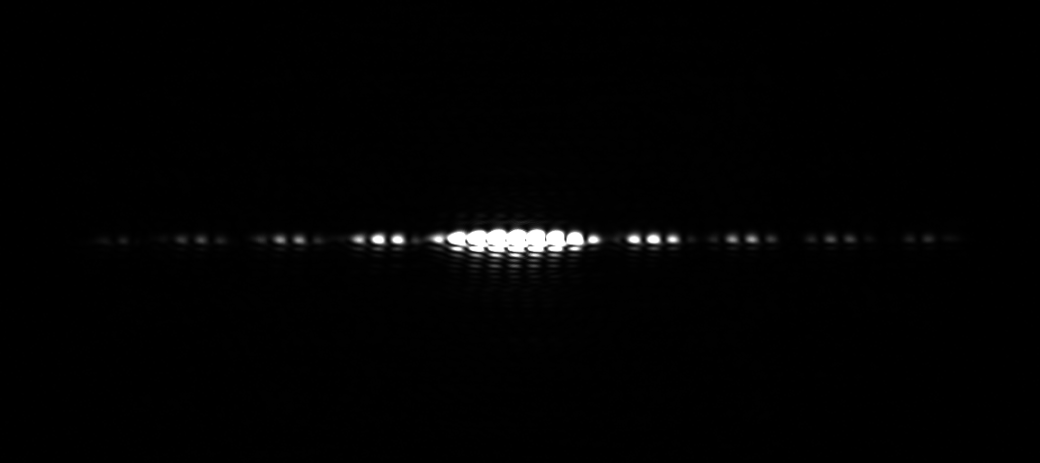
\includegraphics[width=.9\textwidth]{files/3/breit.png}
  \caption{Beugungsbild des breiten Doppelspalts.}
  \label{fig:breit}
\end{figure}


Das Beugungsbild des schmalen Doppelspalts (\abbref{fig:schmal}) zeigte ein sehr breites Hauptmaximum 0. Ordnung, ebenfalls mit etwa drei bis vier Nebenmaxima. Allerdings waren hier fast keine weiteren Hauptmaxima höherer Ordnung zu sehen.

\begin{figure}[H]
  \centering
  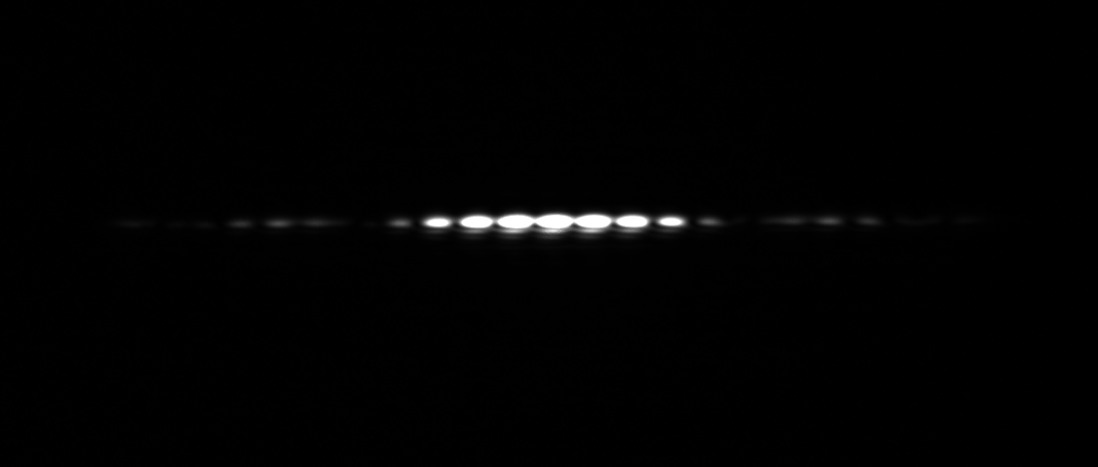
\includegraphics[width=.9\textwidth]{files/3/schmal.png}
  \caption{Beugungsbild des schmalen Doppelspalts.}
  \label{fig:schmal}
\end{figure}


Das Beugungsbild des mittelgroßen Doppelspalts (\abbref{fig:mittel}), bestand aus einem etwas schmaleren Hauptmaximum 0. Ordnung mit etwa drei Nebenmaxima und weiteren weniger gut sichtbaren Hauptmaxima mit etwa einem Nebenmaximum. 

\begin{figure}[H]
  \centering
  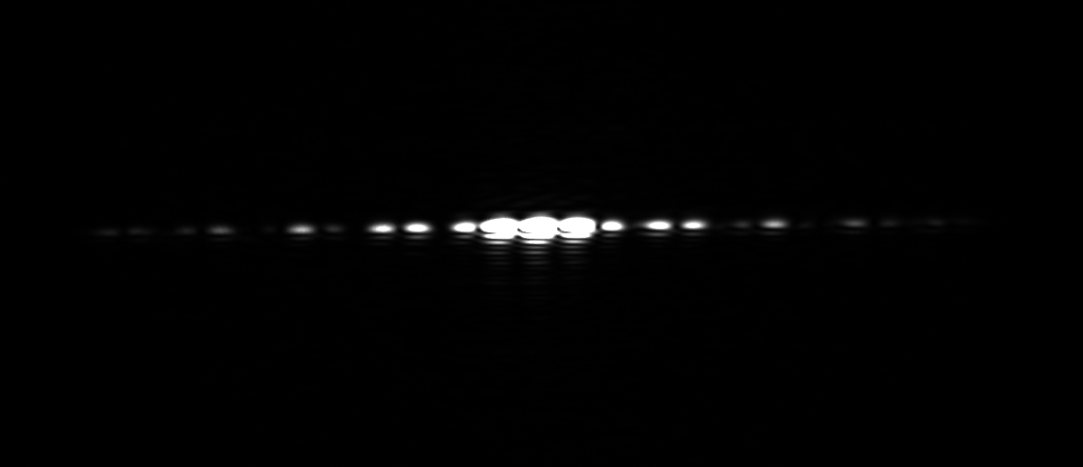
\includegraphics[width=.9\textwidth]{files/3/mittel.png}
  \caption{Beugungsbild des mittleren Doppelspalts.}
  \label{fig:mittel}
\end{figure}

Mit dem mittelgroßen Doppelspalt haben wir auch die weiteren Messungen für diese Aufgabe durchgeführt.

\abbref{fig:ds_theorie_beugungsbild} zeigt das theoretische Beugungsbild des Doppelspalts, generiert mit dem in der Praktikumsanleitung gegebenen Python-Skript. Wir verwenden hierfür den Spaltabstand und die Spaltbreite, wie wir sie in Aufgabe 5 bestimmt haben.

\begin{figure}[H]
  \centering
  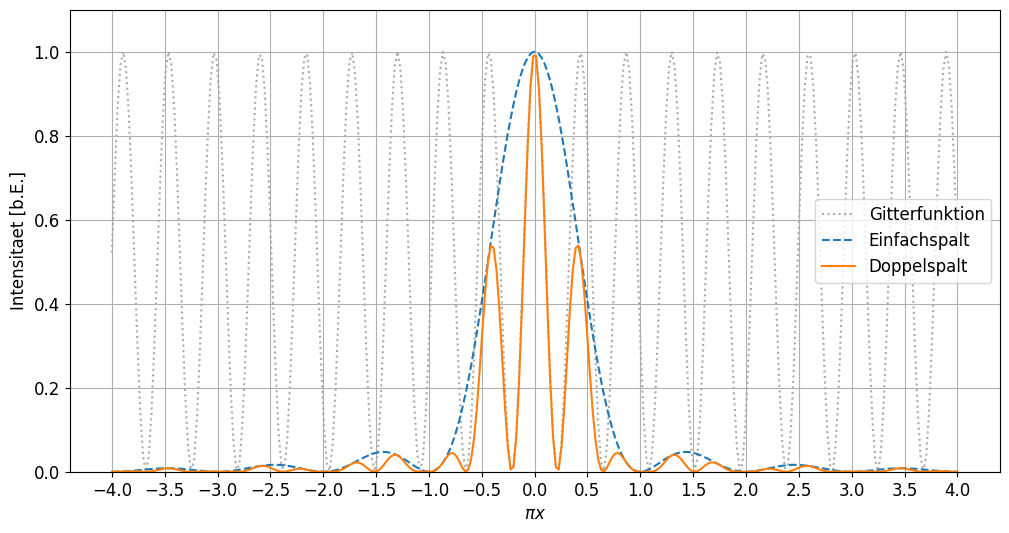
\includegraphics[width=.9\textwidth]{files/plots/3/ds_theorie_beugungsbild.png}
  \caption{Theoretisches Beugungsbild des Doppelspalts mit Funktion des Einzelspalts und Gitterfunktion.}
  \label{fig:ds_theorie_beugungsbild}
\end{figure}

Es ist hier deutlich zu sehen, wie die einhüllende Funktion des Einzelspalts maßgeblich die Form des Beugungsbildes des Doppelspalts beeinflusst. Die Übergänge zwischen den Hauptmaxima bilden sich immer dort, wo sowohl die Gitterfunktion, als auch die Einzelspaltfunktion eine Nullstelle besitzen. Minima innerhalb der Hauptmaxima bilden sich durch Nullstellen der Gitterfunktion, während die Einzelspaltfunktion größer Null ist.

Im Vergleich mit dem gemessenen Beugungsbild zeigen sich, wie zu erwarten, sehr ähnliche Strukturen. Dieses ist in \abbref{fig:ds_gemessen_beugungsbild} zu sehen.

\begin{figure}[H]
  \centering
  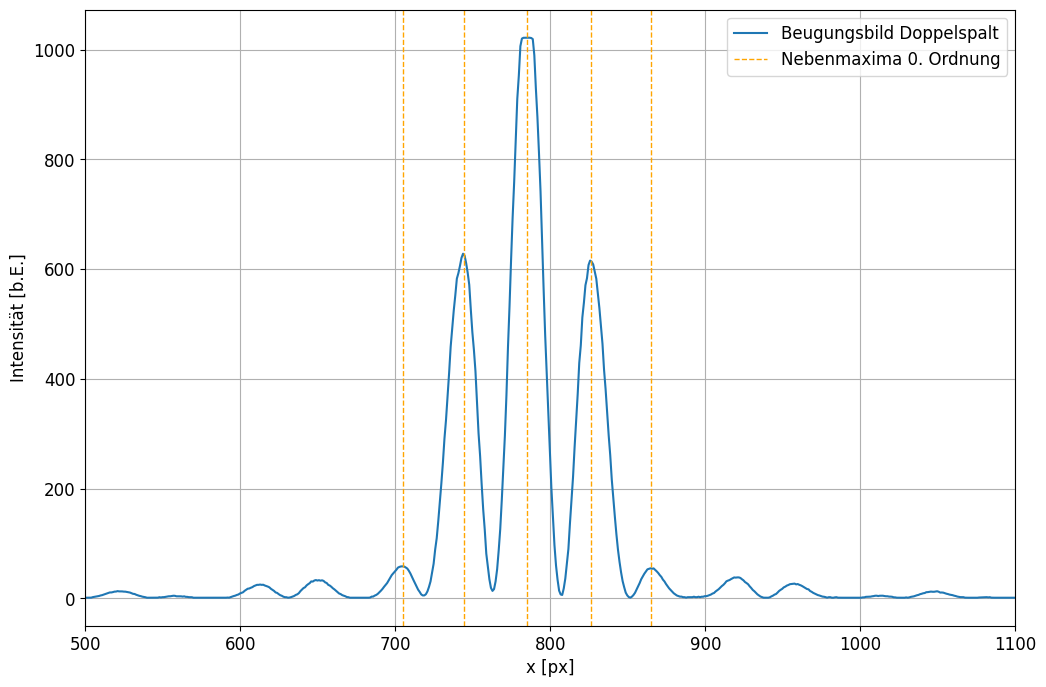
\includegraphics[width=.9\textwidth]{files/plots/3/ds_gemessen_beugungsbild.png}
  \caption{Gemessenes Beugungsbild des Doppelspalts.}
  \label{fig:ds_gemessen_beugungsbild}
\end{figure}

Auch hier sehen wir die fünf Maxima, welche gemeinsam zum mittleren Hauptmaximum 0. Ordnung gehören. Darauf folgt ein breiteres Minimum, welches den Übergang zum Hauptmaximum 1. Ordnung darstellt. In diesem finden sich, wie im theoretischen Bild, zwei kleinere Nebenmaxima.

Wir möchten nun, so wie bereits in Theorie für den Einzelspalt erklärt, die Intensitäten der Nebenmaxima innerhalb der Einhüllenden des nullten Hauptmaximums mit den theoretischen Werten vergleichen. Die Vergleichswerte ermitteln wir wieder numerisch mit dem Online-Grafikrechner, wie in \abbref{fig:ds_intensitaeten_desmos} zu sehen.

Um die Intensitäten vergleichen zu können, berechnen wir zunächst den Normierungsfaktor aus der Intensität des 0. Hauptmaximums
\begin{align}
  N = \frac{1}{I_{0,0}} = (9.78500 \pm 0.00957) \cdot 10^{-4}.
\end{align}

Mit diesem Wert multiplizieren wir nun die Intensität aller in \abbref{fig:ds_gemessen_beugungsbild} Maxima, um so die auf 1 normierten Intensitäten zu erhalten. Diese können wir dann mit den theoretischen Werten vergleichen. Die Resultate des Vergleichs sind in \tabref{tab:es_vergleich_intensitaet} aufgelistet.


\begin{figure}[H]
  \centering
  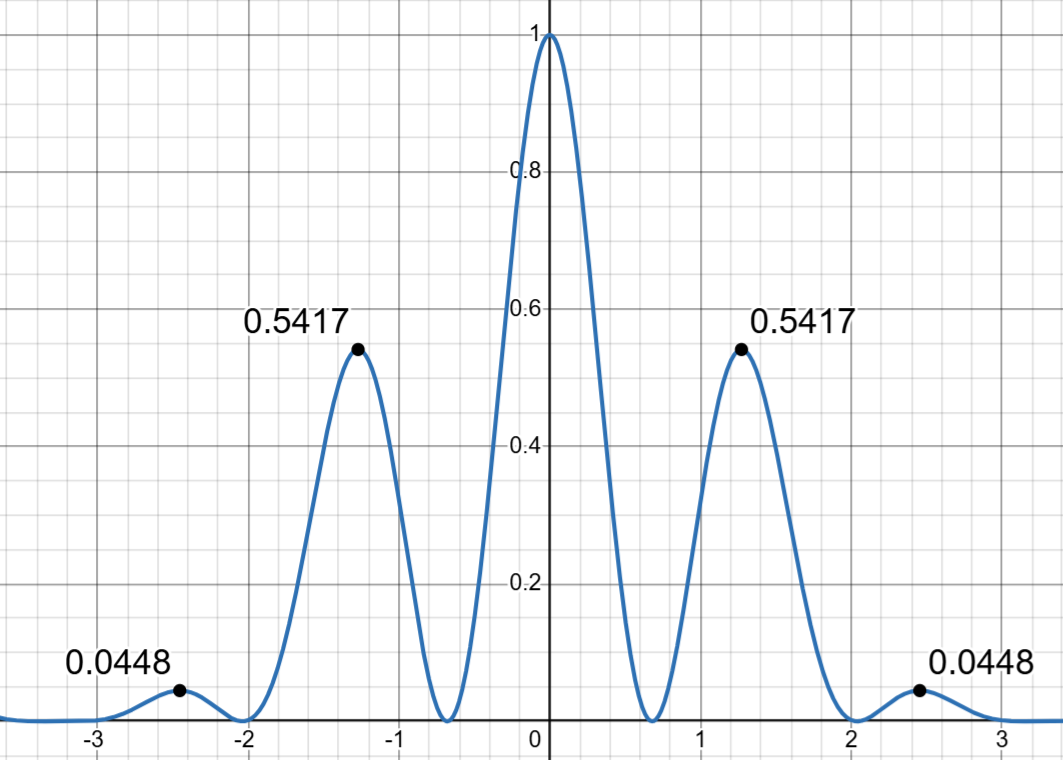
\includegraphics[width=.9\textwidth]{files/plots/3/ds_intensitaeten_desmos.png}
  \caption{Numerische Bestimmung der normierten Intensitäten des 0. Hauptmaximums des Doppelspalts.}
  \label{fig:ds_intensitaeten_desmos}
\end{figure}


\begin{table}[H]
  \centering
  \caption{Vergleich der Intensitäten der Nebenmaxima des 0. Hauptmaximums beim Einzelspalt.}
  \vspace*{0.5em}
  \begin{tabular}{|c|c|c|c|c|}\hline
    Ordnung & Intensität & Intensität (normiert) & Intensität (theo.) & Abw.\\\hline
    \multicolumn{5}{|l|}{Linksseitige Maxima}\\\hline
    1 & $628 \pm 2$   & $0.6146 \pm 0.0021$    &  $0.5417 \pm 0.0001$     &   $35.52\sigma$\\
    2 & $58 \pm 2$    & $0.0568 \pm 0.0020$    &  $0.0448 \pm 0.0001$     &   $6.1\sigma$\\\hline
    \multicolumn{5}{|l|}{Rechtsseitige Maxima}\\\hline
    1 & $616 \pm 2$  &  $0.6028 \pm 0.0021$    &  $0.5417 \pm 0.0001$   &     $29.84\sigma$\\
    2 & $55 \pm 2$   &  $0.0538 \pm 0.0020$    &  $0.0448 \pm 0.0001$   &     $4.61\sigma$\\\hline
  \end{tabular}
  \label{tab:es_vergleich_intensitaet}
\end{table}

\newpage
\subsection{Das Objektbild als Fouriersynthese des Beugungsbildes am Beispiel des Einfachspalts}

Mit der Betrachtung des Objektbilds untersuchen wir in den folgenden beiden Versuchsteilen nun experimentell die Rücktransformation. Der Maßstab der aufgezeichneten Objektbilder wird durch die Linse L1 im Versuchsaufbau beeinflusst. Um aus der Größe $B$ des Bildes die tatsächliche Größe $G$ des Gegenstandes, in diesem Fall das Spaltbild, zu berechnen, ziehen wir zunächst die Linsengleichung
\begin{align}
  \frac{1}{b} + \frac{1}{g} = \frac{1}{f}
\end{align}
heran, welche die Bildweite $b$, die Gegenstandsweite $g$ und die Brennweite $f$ in Verbindung bringt. Mit der Relation
\begin{align}
  \frac{B}{G} = \frac{b}{g}
\end{align}
und der Linsengleichung können wir die Formel
\begin{align}
  \frac{B}{G} = \frac{b - f}{f} = \frac{b}{f} - 1
\end{align}
herleiten. Diese enthält gerade die zwei Werte, Bildweite und Brennweite, welche wir während den Messungen zu diesem Versuchsteil aufgeschrieben haben. Somit können wir einen Umrechnungsfaktor von
\begin{align}
  \frac{B}{G} = 3.38 \pm 0.17
\end{align}
ausrechnen. In unseren Aufzeichnungen geht der Spalt von Pixel $274$ bis Pixel $915$, was mit einem Fehlerwert von $\pm 4$ Pixeln pro Seite, einer Breite von $641 \pm 6 px$ im Bildmaßstab entspricht. Zur Umrechnung von Pixel in Millimeter gibt die Praktikumsanleitung einen Faktor von $3.45 \cdot 10^{-3} \frac{\si{\milli\meter}}{\mathrm{px}}$ an. Multiplizieren wir unseren Wert mit diesem Faktor und teilen durch $\ffrac{B}{G}$, so erhalten wir eine reale Spaltbreite von
\begin{align}
  d = (0.66 \pm 0.04)\si{\milli\meter}.
\end{align}

Nun können wir damit fortfahren, die theoretisch erwarteten Objektbilder zu generieren. Hierzu betrachten wir die Funktion
\begin{align}
  f(k_y, y) = \frac{d}{\pi} \sinc(\frac{kd}{2}) \cos(yk),
\end{align}
welche gerade dem Integranden der Rücktransformation, vorgestellt in der theoretischen Einführung, entspricht. Diese integrieren wir nun numerisch. Dabei setzen wir die untere Integrationsgrenze auf $0$, die obere Grenze auf den Wert
\begin{align}
  k_{y,n} = \frac{2\pi n}{d},
\end{align}
wobei $n$ der Ordnung angibt, bis zu welcher wir integrieren möchten. Die Integration führen wir für $400$ Werte von $y$ im Bereich von $-d$ bis $d$ durch. Abschließend wird das Ergebnis quadriert und die Gesamtmenge der Ergebnisse so normiert, dass der maximale Wert $1$ entspricht.

Wir führen diesen Prozess für die Werte $1, 2, 3, 5$ von $n$ durch, um die theoretischen Objektbilder zu allen von uns aufgezeichneten Bildern zum Vergleich zu erhalten. Zusätzlich setzen wir für einen weiteren Durchgang $n$ auf $51$, um zu sehen, wie sich das tatsächliche Spaltbild im Grenzverhalten $n \to \infty$ ergibt. Die theoretischen Bilder sind in den Abbildungen \ref{fig:es_theorie_objektbild_ord0} bis \ref{fig:es_theorie_objektbild_ord4} zu sehen.

\begin{figure}[H]
  \centering
  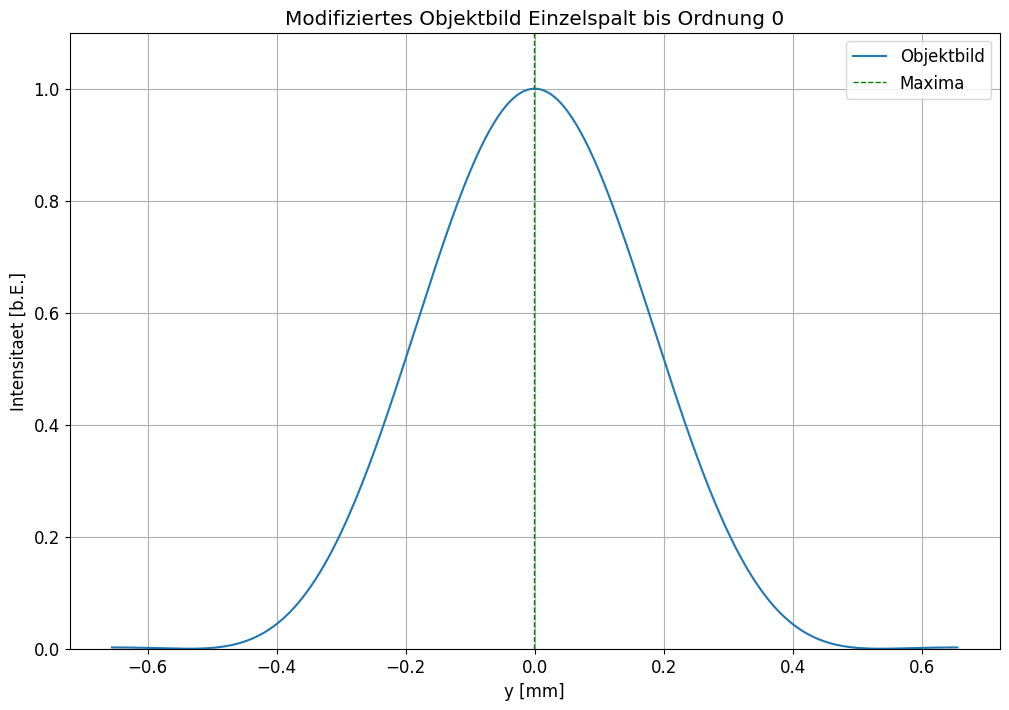
\includegraphics[width=.9\textwidth]{files/plots/4/es_theorie_objektbild_ord0.png}
  \caption{Theoretisches Objektbild aus Rücktransformation bis zur 0. Ordnung.}
  \label{fig:es_theorie_objektbild_ord0}
\end{figure}

\begin{figure}[H]
  \centering
  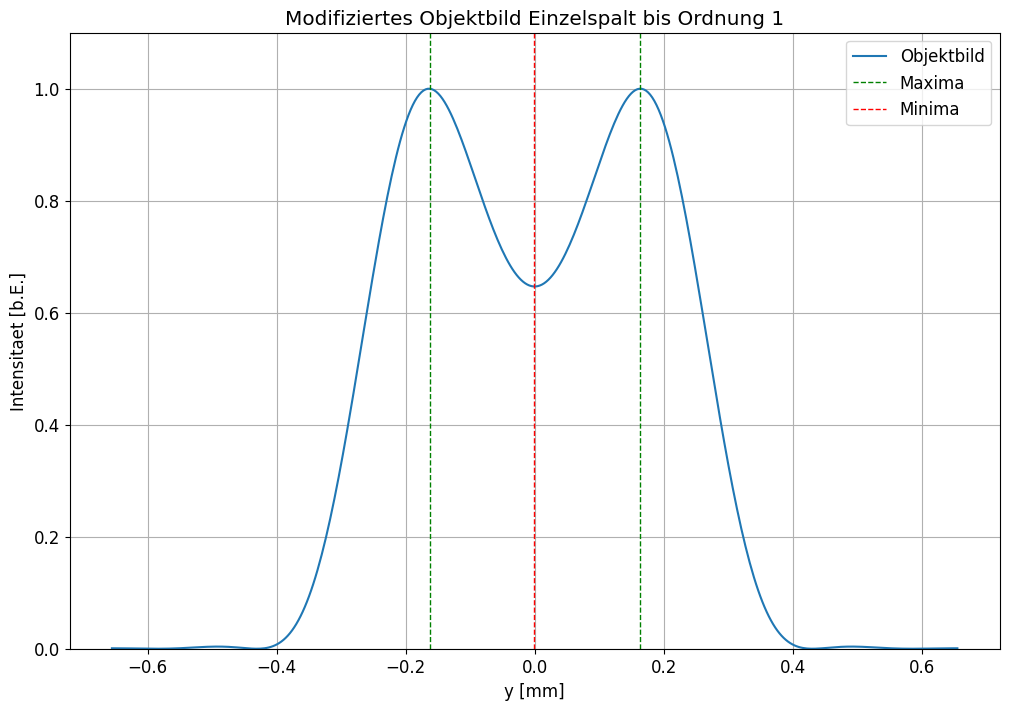
\includegraphics[width=.9\textwidth]{files/plots/4/es_theorie_objektbild_ord1.png}
  \caption{Theoretisches Objektbild aus Rücktransformation bis zur 1. Ordnung.}
  \label{fig:es_theorie_objektbild_ord1}
\end{figure}

\begin{figure}[H]
  \centering
  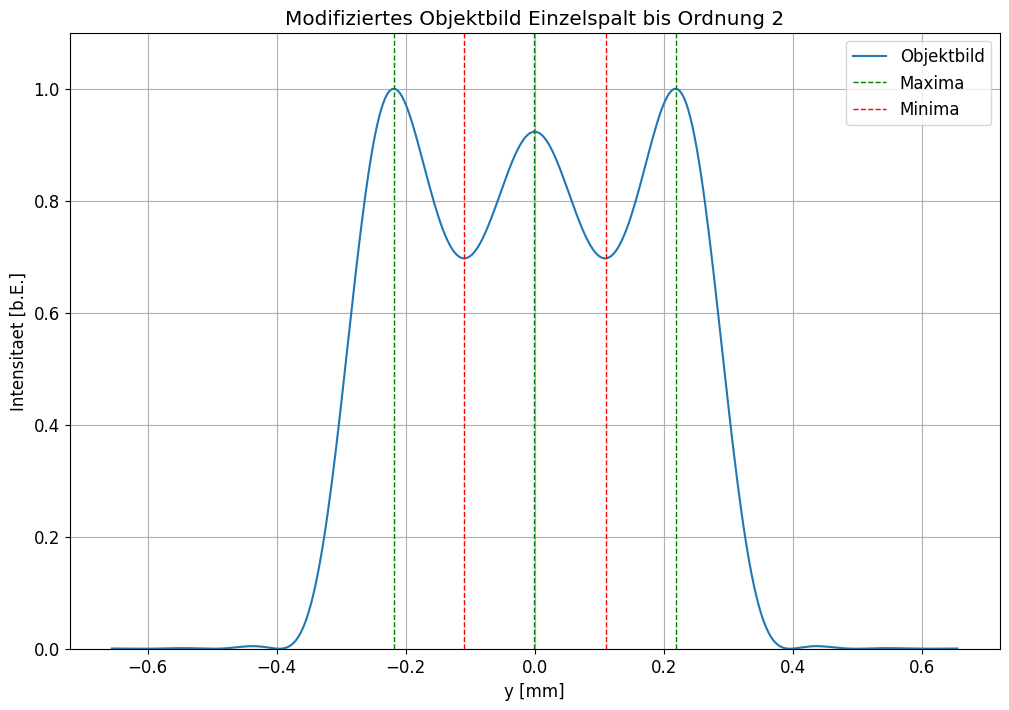
\includegraphics[width=.9\textwidth]{files/plots/4/es_theorie_objektbild_ord2.png}
  \caption{Theoretisches Objektbild aus Rücktransformation bis zur 2. Ordnung.}
  \label{fig:es_theorie_objektbild_ord2}
\end{figure}

\begin{figure}[H]
  \centering
  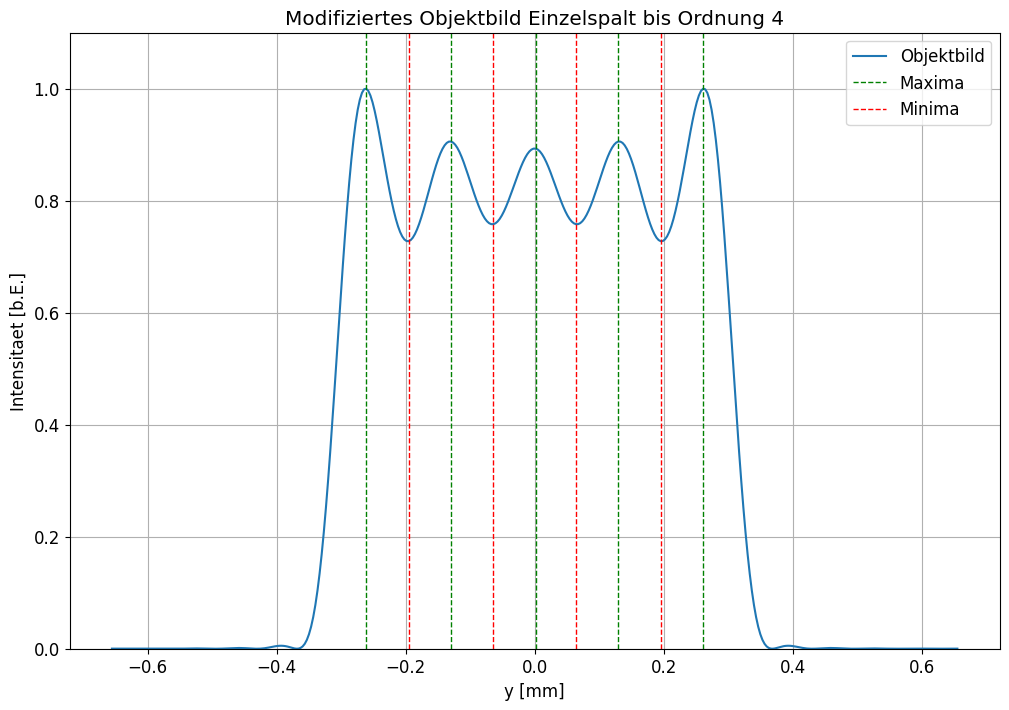
\includegraphics[width=.9\textwidth]{files/plots/4/es_theorie_objektbild_ord4.png}
  \caption{Theoretisches Objektbild aus Rücktransformation bis zur 4. Ordnung.}
  \label{fig:es_theorie_objektbild_ord4}
\end{figure}

Bereits in dieser Abfolge von Plots ist zu sehen, wie mit steigender Ordnung die Kanten steiler und die \glqq{}Wiggles\grqq{} auf dem Plateaubereich kleiner werden und sich das Bild immer näher der rechteckigen Form des Einzelspalts annähert. Besonders deutlich wird dies auf dem Resultat zur Integration bis zu Ordnung $50$ (\abbref{fig:es_theorie_objektbild_ord50}). 

\begin{figure}[H]
  \centering
  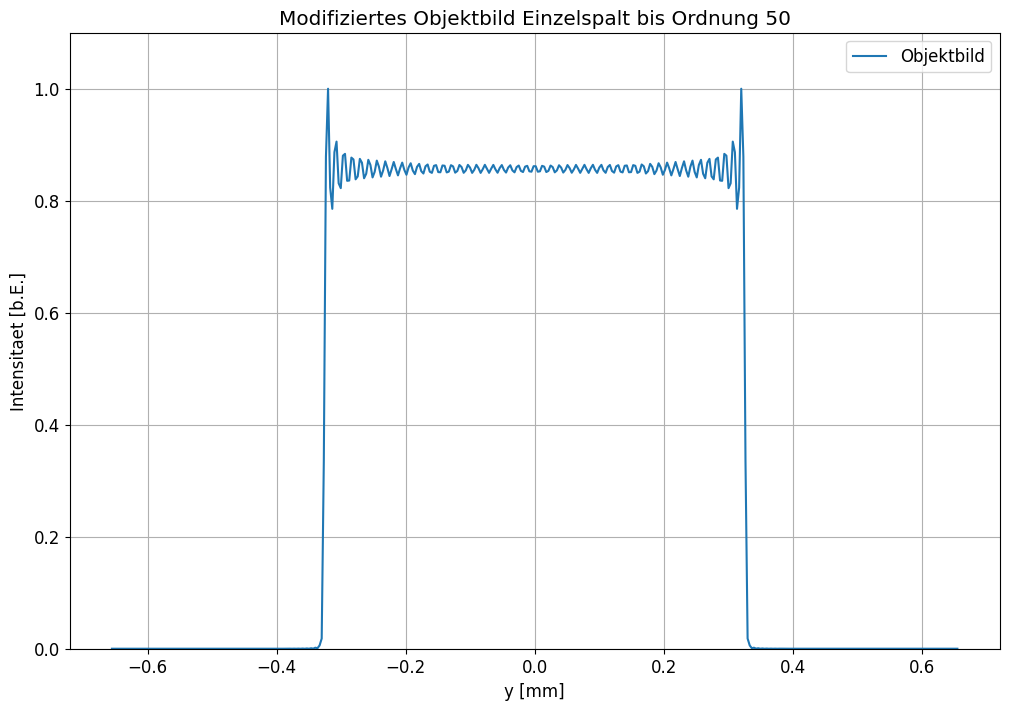
\includegraphics[width=.9\textwidth]{files/plots/4/es_theorie_objektbild_ord50.png}
  \caption{Theoretisches Objektbild aus Rücktransformation bis zur 50. Ordnung.}
  \label{fig:es_theorie_objektbild_ord50}
\end{figure}

Die Theorie möchten wir nun mit den tatsächlich experimentell aufgezeichneten Objektbildern vergleichen. Diese sind in den Abbildungen \ref{fig:es_praxis_objektbild_ord0} bis \ref{fig:es_praxis_objektbild_ord4} dargestellt.

\begin{figure}[H]
  \centering
  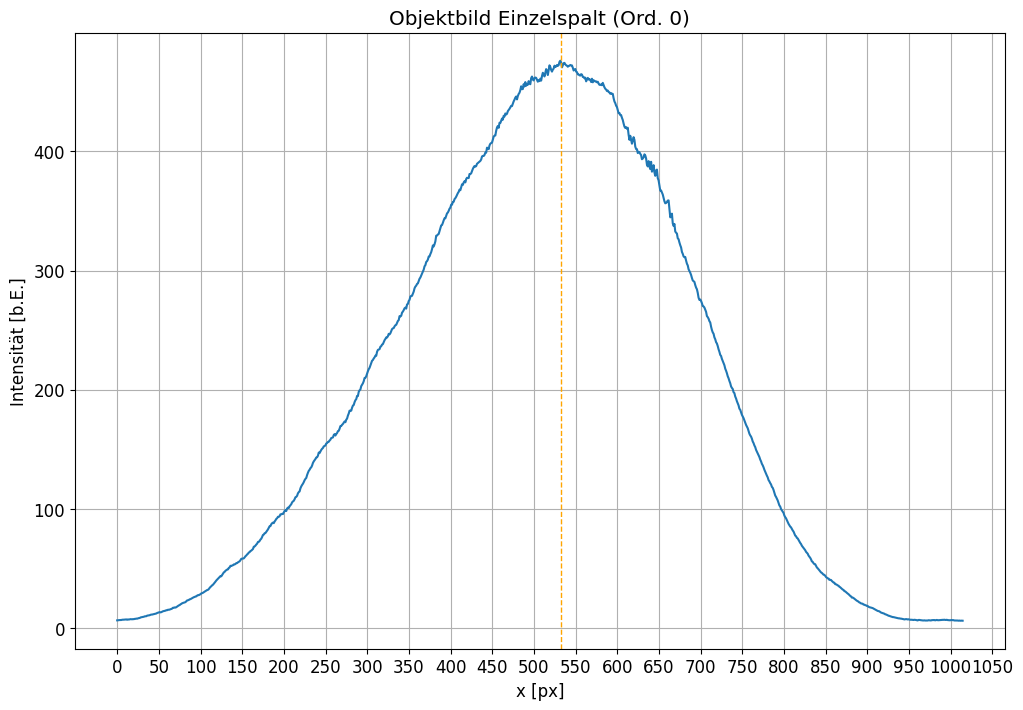
\includegraphics[width=.9\textwidth]{files/plots/4/es_praxis_objektbild_ord0.png}
  \caption{Experimentell bestimmtes Objektbild entsprechend der 0. Ordnung.}
  \label{fig:es_praxis_objektbild_ord0}
\end{figure}

\begin{figure}[H]
  \centering
  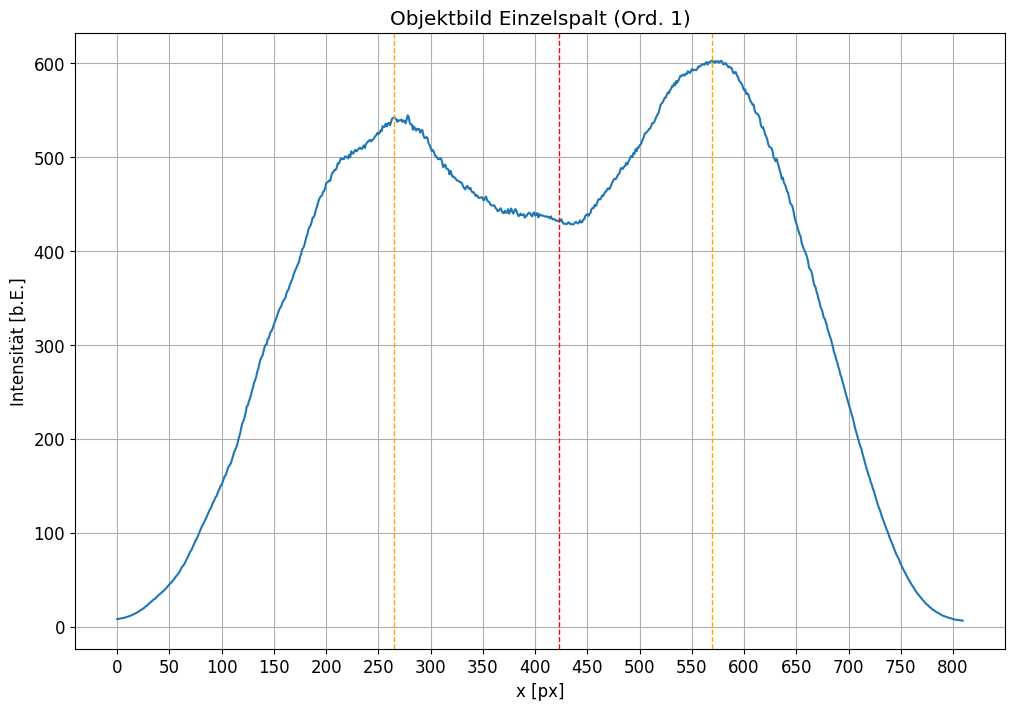
\includegraphics[width=.9\textwidth]{files/plots/4/es_praxis_objektbild_ord1.png}
  \caption{Experimentell bestimmtes Objektbild entsprechend der 1. Ordnung.}
  \label{fig:es_praxis_objektbild_ord1}
\end{figure}

\begin{figure}[H]
  \centering
  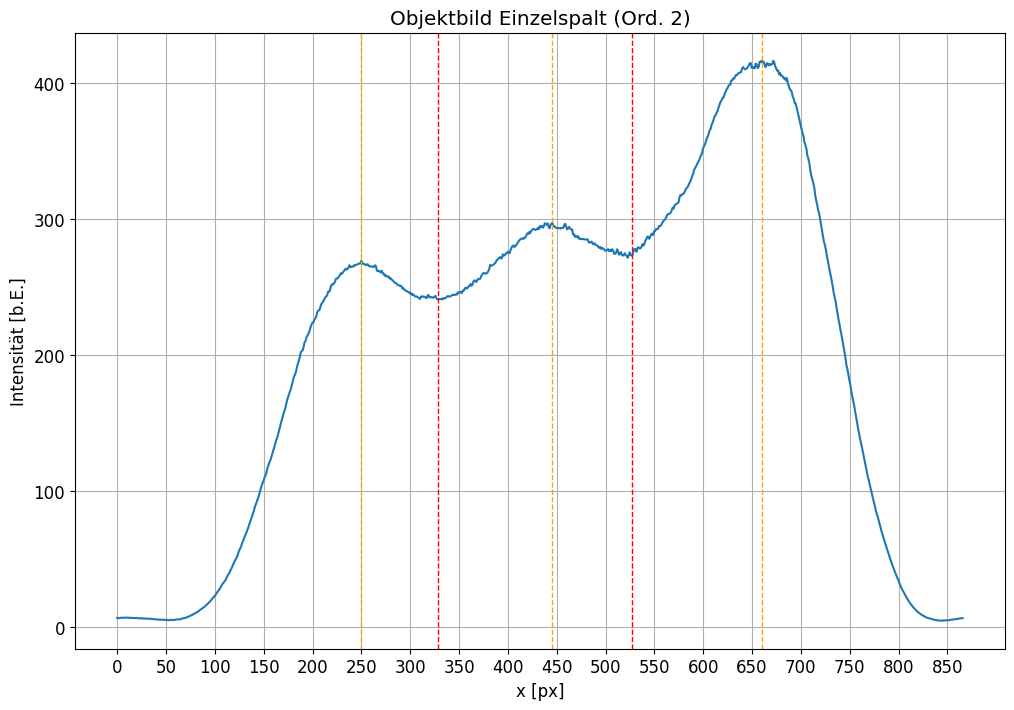
\includegraphics[width=.9\textwidth]{files/plots/4/es_praxis_objektbild_ord2.png}
  \caption{Experimentell bestimmtes Objektbild entsprechend der 2. Ordnung.}
  \label{fig:es_praxis_objektbild_ord2}
\end{figure}

\begin{figure}[H]
  \centering
  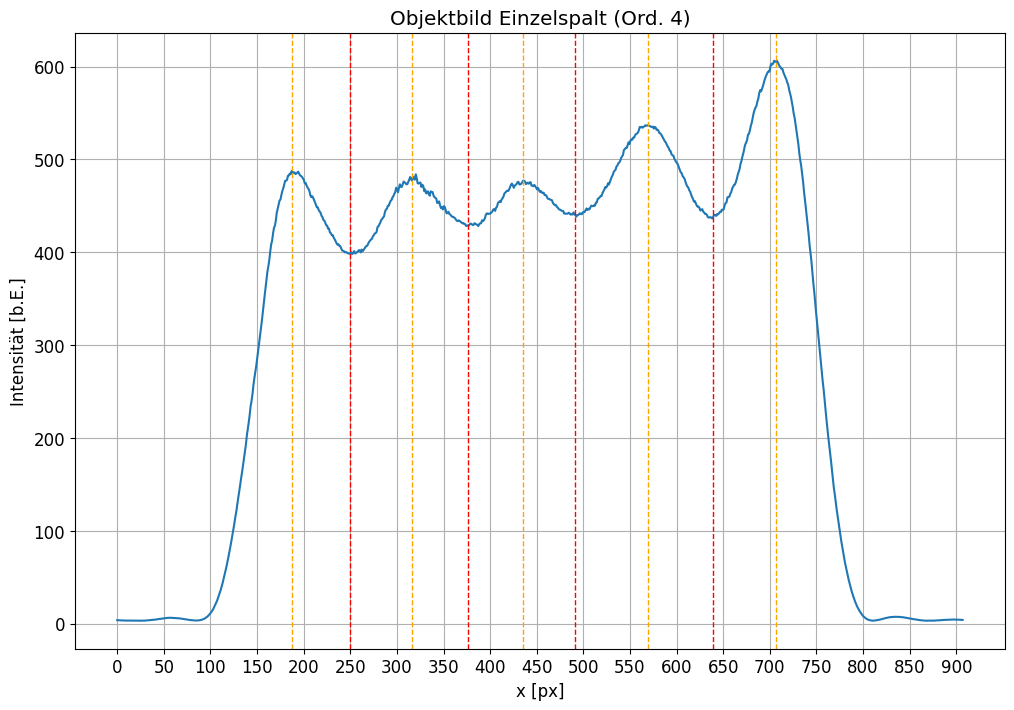
\includegraphics[width=.9\textwidth]{files/plots/4/es_praxis_objektbild_ord4.png}
  \caption{Experimentell bestimmtes Objektbild entsprechend der 4. Ordnung.}
  \label{fig:es_praxis_objektbild_ord4}
\end{figure}

Die experimentell bestimmten Objektbilder zeigen die gleiche Anzahl an Maxima und Minima, wie auch die theoretischen Daten. Während die allerdings die theoretischen Objektbilder in der Intensitätsverteilung immer perfekt Symmetrisch waren, sind bei den experimentell bestimmten Bildern die Maxima verschieden hoch und die Intensität nimmt tendenziell mit aufsteigendem $x$ zu.

Die Abszisse in den Messdaten ist in Pixeln in der Abbildungsebene angegeben. Außerdem sind die Objektbilder hier nicht, wie bei den theoretischen Objektbildern, um den Nullpunkt des Koordinatensystems zentriert. Zum Vergleich der Lage der Maxima und Minima wenden wir deshalb eine relative Betrachtungsweise, bezogen auf das erste Maximum jedes Objektbildes an. Möchten wir beispielsweise die Lage des linken Maximums im Objektbild bis zur ersten Ordnung vergleichen, so gehen wir wie folgt vor:
\begin{enumerate}[label=\arabic*.)]
  \item Lese Lage des 1. Maximums aus $\to x_{0, B}$ (in Pixeln in der Abbildungsebene).
  \item Lese Lage des 2. Maximums aus $\to x_{1, B}$ (in Pixeln in der Abbildungsebene).
  \item Berechne Distanz der beiden Werte $x_{\overline{01}, B} = |x_{1} - x_{0}|$ (in Pixeln in der Abbildungsebene).
  \item Berechne reale Distanz der Maxima $x_{\overline{01}, G} = x_{\overline{01}, B} \cdot \ffrac{3.45 \cdot 10^{-3} \frac{\si{\milli\meter}}{\mathrm{px}}}{\frac{B}{G}}$.
  \item Berechne Distanz der beiden Maxima im theoretischen Objektbild (in $\si{\milli\meter}$ in der Gegenstandsebene).
  \item Vergleiche die beiden Werte.
\end{enumerate} 

Da diese Methode des Vergleichs immer mindestens zwei Maxima benötigt, können wir damit logischerweise erst beim Objektbild 1. Ordnung beginnen.

Die folgenden Tabellen \ref{tab:vergl_objbild_ma_mi_x_ord1} bis \ref{tab:vergl_objbild_ma_mi_x_ord4} fassen die Ergebnisse zum Vergleich der Lage der Maxima und Minima zusammen.

\newpage

\begin{table}[H]
  \centering
  \caption{Vergleich der Lage der Maxima und Minima im experimentell bestimmten Objektbild 1. Ordnung mit der Theorie.}
  \vspace*{0.5em}
  \begin{tabular}{|c|c|c|c|c|c|c|}\hline
    \multirow{2}{*}{\#} & \multicolumn{3}{c|}{Praxis} & \multicolumn{2}{c|}{Theorie} & \multirow{2}{*}{Abw.}\\\cline{2-6}
        & Pos. [px] & $\Delta$ 1. Max [px] & $\Delta$ Umger. [mm] & Pos. [mm] & $\Delta$1. Max [mm] & \\\hline
    \multicolumn{7}{|l|}{Maxima}\\\hline
    1   & $265 \pm 4$ & -                 & -             & $-0.16$ & -                 & - \\
    2   & $ 569 \pm 4$ & $304 \pm 6$ & $0.311 \pm 0.006$ & $0.16$ & $0.33$ & $2.5\sigma$\\\hline
    \multicolumn{7}{|l|}{Minima}\\\hline
    1   & $423 \pm 4$ & $158 \pm 6$ & $0.162 \pm 0.006$ & $0.00$ & $0.16$ & $0.1\sigma$\\\hline
  \end{tabular}
  \label{tab:vergl_objbild_ma_mi_x_ord1}
\end{table}
\begin{table}[H]
  \centering
  \caption{Vergleich der Lage der Maxima und Minima im experimentell bestimmten Objektbild 2. Ordnung mit der Theorie.}
  \vspace*{0.5em}
  \begin{tabular}{|c|c|c|c|c|c|c|}\hline
    \multirow{2}{*}{\#} & \multicolumn{3}{c|}{Praxis} & \multicolumn{2}{c|}{Theorie} & \multirow{2}{*}{Abw.}\\\cline{2-6}
        & Pos. [px] & $\Delta$ 1. Max [px] & $\Delta$ Umger. [mm] & Pos. [mm] & $\Delta$1. Max [mm] & \\\hline
    \multicolumn{7}{|l|}{Maxima}\\\hline
    1   & $250 \pm 4$ & -                 & -             & $-0.22$ & -                 & - \\
    2   & $445 \pm 4$ & $195 \pm 6$ & $0.200 \pm 0.006$ & $0.0$ & $0.22$ & $3.02\sigma$\\
    3   & $660 \pm 4$ & $410 \pm 6$ & $0.420 \pm 0.006$ & $0.22$ & $0.44$ & $3.07\sigma$\\\hline
    \multicolumn{7}{|l|}{Minima}\\\hline
    1   & $328 \pm 4$ & $78 \pm 6$ & $0.080 \pm 0.006$ & $-0.11$ & $0.11$ & $4.96\sigma$\\
    2   & $527 \pm 4$ & $277 \pm 6$ & $0.283 \pm 0.006$ & $0.11$ & $0.33$ & $7.84\sigma$\\\hline
  \end{tabular}
  \label{tab:vergl_objbild_ma_mi_x_ord2}
\end{table}
\begin{table}[H]
  \centering
  \caption{Vergleich der Lage der Maxima und Minima im experimentell bestimmten Objektbild 4. Ordnung mit der Theorie.}
  \vspace*{0.5em}
  \begin{tabular}{|c|c|c|c|c|c|c|}\hline
    \multirow{2}{*}{\#} & \multicolumn{3}{c|}{Praxis} & \multicolumn{2}{c|}{Theorie} & \multirow{2}{*}{Abw.}\\\cline{2-6}
        & Pos. [px] & $\Delta$ 1. Max [px] & $\Delta$ Umger. [mm] & Pos. [mm] & $\Delta$1. Max [mm] & \\\hline
    \multicolumn{7}{|l|}{Maxima}\\\hline
    1   & $187 \pm 4$ & -                 & -             & $-0.26$ & -                 & - \\
    2   & $316 \pm 4$ & $129 \pm 6$ & $0.132 \pm 0.006$ & $-0.13$ & $0.13$ & $0.09\sigma$\\
    3   & $435 \pm 4$ & $248 \pm 6$ & $0.254 \pm 0.006$ & $0.00$ & $0.26$ & $1.6\sigma$\\
    4   & $569 \pm 4$ & $382 \pm 6$ & $0.391 \pm 0.006$ & $0.13$ & $0.40$ & $0.07\sigma$\\
    5   & $707 \pm 4$ & $520 \pm 6$ & $0.532 \pm 0.006$ & $0.26$ & $0.52$ & $1.62\sigma$\\\hline
    \multicolumn{7}{|l|}{Minima}\\\hline
    1   & $250 \pm 4$ & $63 \pm 6$  & $0.064 \pm 0.006$ & $-0.20$ & $0.07$ & $0.23\sigma$\\
    2   & $376 \pm 4$ & $189 \pm 6$ & $0.193 \pm 0.006$ & $-0.06$ & $0.20$ & $0.67\sigma$\\
    3   & $491 \pm 4$ & $304 \pm 6$ & $0.311 \pm 0.006$ & $0.06$  & $0.33$ & $2.5\sigma$\\
    4   & $639 \pm 4$ & $452 \pm 6$ & $0.462 \pm 0.006$ & $0.20$ & $0.46$ & $0.96\sigma$\\\hline
  \end{tabular}
  \label{tab:vergl_objbild_ma_mi_x_ord4}
\end{table}

\newpage

Die nachfolgenden Tabellen \ref{tab:vergl_objbild_ma_mi_i_ord1} bis \ref{tab:vergl_objbild_ma_mi_i_ord4} zeigen die Resultate der Vergleiche der Intensitäten der Maxima und Minima. Um die Intensitäten zu vergleichen, müssen wir nicht mit den Maßstäben der Abszisse herumrechnen. Hier normieren wir aber zur Vergleichbarkeit die Intensitäten so, dass die Intensität des ersten Maximums $1$ entspricht.

\begin{table}[H]
  \centering
  \caption{Vergleich der Intensität der Maxima und Minima im experimentell bestimmten Objektbild 1. Ordnung mit der Theorie.}
  \vspace*{0.5em}
  \begin{tabular}{|c|c|c|c|c|}\hline
    \multirow{2}{*}{\#} & \multicolumn{2}{c|}{Praxis} & \multicolumn{1}{c|}{Theorie} & \multirow{2}{*}{Abw.}\\\cline{2-4}
        & I [b.E.] & I norm. auf 1. Max & I [b.E.] & \\\hline
    \multicolumn{5}{|l|}{Maxima}\\\hline
    1   & $543 \pm 2$ & -                             & $1.0$& - \\
    2   & $603 \pm 2$ & $1.111 \pm 0.006$ & $1.0$  & $20.08\sigma$\\\hline
    \multicolumn{5}{|l|}{Minima}\\\hline
    1   & $432 \pm 2$ & $0.795 \pm 0.005$ & $0.65$ & $31.48\sigma$\\\hline
  \end{tabular}
  \label{tab:vergl_objbild_ma_mi_i_ord1}
\end{table}

\begin{table}[H]
  \centering
  \caption{Vergleich der Intensität der Maxima und Minima im experimentell bestimmten Objektbild 2. Ordnung mit der Theorie.}
  \vspace*{0.5em}
  \begin{tabular}{|c|c|c|c|c|}\hline
    \multirow{2}{*}{\#} & \multicolumn{2}{c|}{Praxis} & \multicolumn{1}{c|}{Theorie} & \multirow{2}{*}{Abw.}\\\cline{2-4}
        & I [b.E.] & I norm. auf 1. Max & I [b.E.] & \\\hline
    \multicolumn{5}{|l|}{Maxima}\\\hline
    1   & $270 \pm 2$ & -                             & $1.0$               & - \\
    2   & $297 \pm 2$ & $1.103 \pm 0.012$ & $0.92$ &  $16.25\sigma$\\
    3   & $416 \pm 2$ & $1.547 \pm 0.014$ & $1.0$ & $39.98\sigma$\\\hline
    \multicolumn{5}{|l|}{Minima}\\\hline
    1   & $241 \pm 2$ & $0.896 \pm 0.010$ & $0.70$ & $19.90\sigma$\\
    2   & $273 \pm 2$ & $1.015 \pm 0.011$ & $0.70$ & $30.05\sigma$\\\hline
  \end{tabular}
  \label{tab:vergl_objbild_ma_mi_i_ord2}
\end{table}

\begin{table}[H]
  \centering
  \caption{Vergleich der Intensität der Maxima und Minima im experimentell bestimmten Objektbild 4. Ordnung mit der Theorie.}
  \vspace*{0.5em}
  \begin{tabular}{|c|c|c|c|c|}\hline
    \multirow{2}{*}{\#} & \multicolumn{2}{c|}{Praxis} & \multicolumn{1}{c|}{Theorie} & \multirow{2}{*}{Abw.}\\\cline{2-4}
        & I [b.E.] & I norm. auf 1. Max & I [b.E.] & \\\hline
    \multicolumn{5}{|l|}{Maxima}\\\hline
    1 & $488 \pm 2$ & - & $1.0$ & - \\
    2 & $477 \pm 2$ & $0.97888 \pm 0.006$ & $0.91$ &  $12.76\sigma$ \\
    3 & $477 \pm 2$ & $0.97867 \pm 0.006$ & $0.89$ &  $14.92\sigma$ \\
    4 & $537 \pm 2$ & $1.10152 \pm 0.007$ & $0.91$ &  $32.10\sigma$ \\
    5 & $605 \pm 2$ & $1.24118 \pm 0.007$ & $1.0$ &  $36.90\sigma$ \\\hline
    \multicolumn{5}{|l|}{Minima}\\\hline
    1 & $398 \pm 2$ & $0.817 \pm 0.006$ & $0.73$ & $16.83\sigma$ \\
    2 & $429 \pm 2$ & $0.880 \pm 0.006$ & $0.76$ & $22.28\sigma$ \\
    3 & $441 \pm 2$ & $0.904 \pm 0.006$ & $0.76$ & $26.33\sigma$ \\
    4 & $437 \pm 2$ & $0.895 \pm 0.006$ & $0.73$ & $30.43\sigma$ \\\hline
  \end{tabular}
  \label{tab:vergl_objbild_ma_mi_i_ord4}
\end{table}


%\begin{table}[H]
%  \centering
%  \begin{tabular}{|c|c|c|c|c|c|c|}\hline
%    \multirow{2}{*}{\#} & \multicolumn{3}{c|}{Praxis} & \multicolumn{2}{c|}{Theorie} & \multirow{2}{*}{Abw.}\\\cline{2-6}
%        & Pos. [px] & $\Delta$ 1. Max [px] & $\Delta$ Umger. [mm] & Pos. [mm] & $\Delta$1. Max [mm] & \\\hline
%    \multicolumn{7}{|l|}{Maxima}\\\hline
%    1   & $$ & -                 & -             & $$ & -                 & - \\
%    2   & $$ & $$ & $$ & $$ & $$ & $$\\\hline
%    \multicolumn{7}{|l|}{Minima}\\\hline
%    1   & $$ & $$ & $$ & $$ & $$ & $$\\\hline
%  \end{tabular}
%\end{table}